\documentclass[12pt]{article}
\usepackage[margin=2.5cm]{geometry}
\usepackage{enumerate}
\usepackage{amsfonts}
\usepackage{amsmath}
\usepackage{fancyhdr}
\usepackage{amsmath}
\usepackage{amssymb}
\usepackage{amsthm}
\usepackage{mdframed}
\usepackage{graphicx}
\usepackage{subcaption}
\usepackage{adjustbox}
\usepackage{listings}
\usepackage{xcolor}
\usepackage{booktabs}
\usepackage[utf]{kotex}
\usepackage{hyperref}
\usepackage{accents}

\definecolor{codegreen}{rgb}{0,0.6,0}
\definecolor{codegray}{rgb}{0.5,0.5,0.5}
\definecolor{codepurple}{rgb}{0.58,0,0.82}
\definecolor{backcolour}{rgb}{0.95,0.95,0.92}

\lstdefinestyle{mystyle}{
    backgroundcolor=\color{backcolour},
    commentstyle=\color{codegreen},
    keywordstyle=\color{magenta},
    numberstyle=\tiny\color{codegray},
    stringstyle=\color{codepurple},
    basicstyle=\ttfamily\footnotesize,
    breakatwhitespace=false,
    breaklines=true,
    captionpos=b,
    keepspaces=true,
    numbers=left,
    numbersep=5pt,
    showspaces=false,
    showstringspaces=false,
    showtabs=false,
    tabsize=1
}

\lstset{style=mystyle}

\pagestyle{fancy}
\renewcommand{\headrulewidth}{0.4pt}
\lhead{CSC 343}
\rhead{Worksheet 10 Solution}

\begin{document}
\title{CSC343 Worksheet 10 Solution}
\maketitle

\bigskip

\begin{enumerate}[1.]
    \item

    \begin{enumerate}[a)]

        \item /Products/Maker/PC/RAM

        \bigskip

        \underline{\textbf{Notes:}}

        \begin{itemize}
            \item XPATH and Selecting Nodes
            \begin{itemize}
                \item nodename
                \begin{itemize}
                    \item Selects all nodes with the name "nodename"
                \end{itemize}
                \item /
                \begin{itemize}
                    \item Selects from the root node
                \end{itemize}
                \item //
                \begin{itemize}
                    \item Selects node in the document from the current node that
                    match the selection no matter where they are
                \end{itemize}
                \item .
                \begin{itemize}
                    \item Select the current node
                \end{itemize}
                \item ..
                \begin{itemize}
                    \item Selects the parent of the current node
                \end{itemize}
                \item @
                \begin{itemize}
                    \item Selects attributes
                \end{itemize}
            \end{itemize}

            \bigskip

            \underline{\textbf{Example:}}

    \begin{lstlisting}[language=XML]
    /StarMovieData/Star//City
    \end{lstlisting}

            \bigskip

            \begin{itemize}
                \item selects all City element in

                \bigskip

                $<$StarMovieData$>$

                \quad$<$Star$>$

                \quad\quad\textit{Here :)}

                \quad$<$/Star$>$

                $<$/StarMovieData$>$
            \end{itemize}

            \item Wildcards *
            \begin{itemize}
                \item Is used to say 'any tag'
            \end{itemize}

            \bigskip

            \underline{\textbf{Example:}}

            \bigskip

    \begin{lstlisting}[language=XML]
    /StarMovieData/*/@*
    \end{lstlisting}

            \bigskip

            \begin{itemize}
                \item `@*' means any attributes
                \item `*' means any tag
            \end{itemize}
            \item Context of Expressions
            \begin{itemize}
                \item $[...]$ means that exists or there exists
                \item $[\textit{integer}]$ selects ith child of its parent
                \item $[\textit{Tag}]$ selects elements that have one or more sublements with `Tag'
                \item$[\textit{Attribute}]$ selects elements that have attribute `Attribute'

                \bigskip

                \underline{\textbf{Example:}}

                \bigskip

    \begin{lstlisting}[language=XML]
    /StarMovieData/Star[//City = "Malibu"]/Name
    \end{lstlisting}

                \bigskip

                \begin{itemize}
                    \item Means select all Star Name that contains City with value `Malibu'
                \end{itemize}

                \bigskip

                \underline{\textbf{Example:}}

    \begin{lstlisting}
    /Movies/Movie/Version[1]/@year
    \end{lstlisting}

                \bigskip

                \begin{itemize}
                    \item Returns value of `year' attribute of first `Version' tag in `Movie'
                    \item e.g. 1933 and 1984

                    \bigskip

                    \begin{center}
                    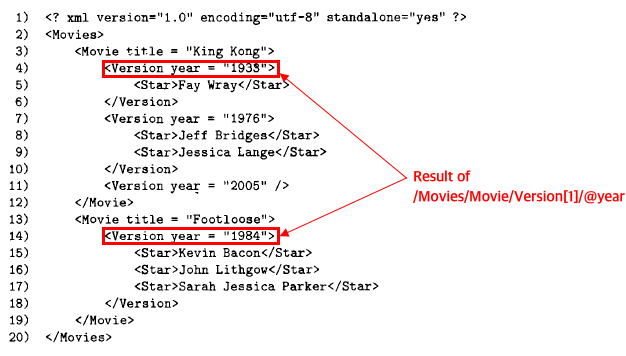
\includegraphics[width=\linewidth]{images/worksheet_10_3.png}
                    \end{center}
                \end{itemize}

                \bigskip

                \underline{\textbf{Example 2:}}


    \begin{lstlisting}
    /Movies/Movie/Version
    \end{lstlisting}

                \bigskip

                \begin{itemize}
                    \item Returns all `Version' tag in `Movie'
                    \item e.g. lines 4 through 6, 7 through 10, line 11, lines 14 through 18

                    \bigskip

                    \begin{center}
                    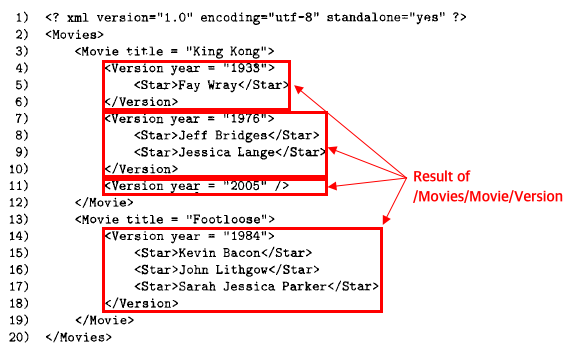
\includegraphics[width=\linewidth]{images/worksheet_10_4.png}
                    \end{center}
                \end{itemize}

                \bigskip

                \underline{\textbf{Example 3:}}


    \begin{lstlisting}
    /Movies/Movie/Version[Star]
    \end{lstlisting}

                \bigskip

                \begin{itemize}
                    \item Selects all `Version' tag with one or more `Star' tag inside
                    \item e.g lines 4 through 6, 7 through 10, 14 through 18

                    \begin{center}
                    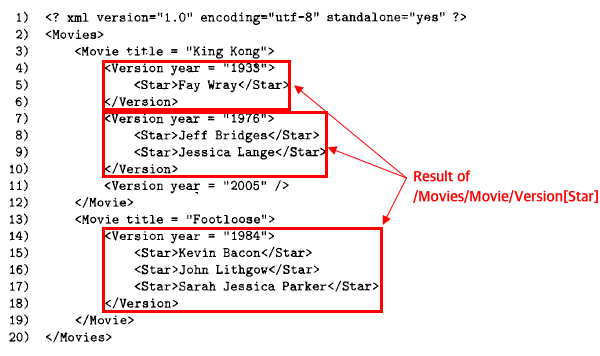
\includegraphics[width=\linewidth]{images/worksheet_10_5.png}
                    \end{center}
                \end{itemize}
            \end{itemize}

        \end{itemize}

        \item /Products/Maker/*/@price
        \item /Products/Maker/Printer
        \item /Products/Maker[/Printer/Type/text() = 'ink-jet']

        \bigskip

        \begin{mdframed}
            \underline{\textbf{Correct Solution:}}

            /Products/Maker[Printer/Type/text() = 'ink-jet']

        \end{mdframed}
        \item /Products/Maker[/PC $\vert$ /Laptops]

        \bigskip

        \underline{\textbf{Notes:}}

        \bigskip

        \begin{itemize}
            \item XPATH and OR
            \begin{itemize}
                \item \textbf{Syntax:} (\textit{xpath expression 1}) $\vert$ (\textit{xpath expression 2}) $^{[1]}$
            \end{itemize}
        \end{itemize}

        \bigskip

        \underline{\textbf{References:}}

        \bigskip

        \begin{enumerate}[1)]
            \item Stack Overflow, XPath OR operator for different nodes, \href{https://stackoverflow.com/questions/5350666/xpath-or-operator-for-different-nodes}{link}
        \end{enumerate}

        \item /Products/Maker/*[HardDisk/text() $>$ 200]/@model
    \end{enumerate}

    \item

    \begin{enumerate}[a)]
        \item /Ships/Class/Ship/@name
        \item /Ships/Class[@displacement $>$ 35000]
        \item /Ships/Class/Ship[@launched $<$ 1917]
        \item /Ships/Class/Ship[Battle/@outcome = 'sunk']/@name
        \item /Ships[Class/@name = Class/Ship/@name]/Class/Ship/@launched
        \item /Ships/Class/Ship[Battle]/@name
    \end{enumerate}

    \item

    \begin{enumerate}[a)]
        \item

        \bigskip

        \underline{\textbf{Notes:}}

        \bigskip

        \begin{itemize}
            \item XQuery
            \begin{itemize}
                \item Means \textbf{XML Query}
                \item Is a functional language
            \end{itemize}
            \item XQuery and FLWOR
            \begin{itemize}
                \item FLWOR means
                \begin{enumerate}[1.]
                    \item \textbf{F}or - selects a sequence of nodes
                    \item \textbf{L}et - binds a sequence to a variable
                    \item \textbf{W}here - filters the nodes
                    \item \textbf{O}rder By - sorts the nodes
                    \item \textbf{R}eturn - what to return (gets evaluated once for every node)

                    \bigskip

                    \underline{\textbf{Example:}}

                    \bigskip

    \begin{lstlisting}
    doc("books.xml")/bookstore/book[price>30]/title

    for $x in doc("books.xml")/bookstore/book
    where $x/price>30
    return $x/title
    \end{lstlisting}

                \end{enumerate}
                \item \textbf{Let} cluase
                \begin{itemize}
                    \item \textbf{Syntax:} let \textit{variable} := \textit{expression}
                    \item Has a use case of storing document

                    \bigskip

                    e.g.

                    \bigskip

                    \$stars := doc('stars.xml');

                \end{itemize}

                \item \textbf{For} cluase

                \begin{itemize}
                    \item \textbf{Syntax:} for \textit{variable} in \textit{expression}

                    \bigskip

                    \underline{\textbf{Example:}}

    \begin{lstlisting}
    let $movies := doc("movies.xml");
    for $m in $movies/Movies/Movie
    where $/@title = 'King Kong'
    return $m
    \end{lstlisting}
                \end{itemize}

                \item \textbf{Where} Clause
                \begin{itemize}
                    \item \textbf{Syntax:} \textbf{where} \textit{condition}
                \end{itemize}

                \item \textbf{Return} Clause
                \begin{itemize}
                    \item \textbf{Syntax:} \textbf{return} \textit{expression}
                \end{itemize}

            \end{itemize}

            \item Replacement of Variables
            \begin{itemize}
                \item Is done using curly braces $\{\}$

                \bigskip

                \underline{\textbf{Example:}}

    \begin{lstlisting}
    let $movies := doc("movies.xml");
    for $m in $movies/Movies/Movie
    return <Movie title= {$/@title}>{$m/Version/Star}</Movie>
    \end{lstlisting}
            \end{itemize}

        \end{itemize}

    \end{enumerate}
\end{enumerate}

\end{document}